\section{Localization system}

This section details the ROS implementation of the proposed 3/6 DoF self-localization system\footnote{\url{https://github.com/carlosmccosta/dynamic_robot_localization}}. It starts with an overview of the main processing stages and then details the control flow and algorithms within the localization pipeline.

\subsection{Overview}

The self-localization system was implemented as a \gls{ros} package and provides 3/6 \gls{dof} localization by publishing \emph{geometry\_msgs::PoseStamped} and \emph{geometry\_msgs::TransformStamped} messages along with a detailed analysis of the pose estimation and registered point cloud (split into inliers and outliers). Moreover, it also gives detailed analysis of the computation runtime of each of its modules in order to pinpoint which algorithms are using more computation resources, which is very useful information when configuring or upgrading the system.

The \gls{ros} implementation can receive sensor data through \emph{sensor\_msgs::PointCloud2} messages and as a result it can directly use data from RGB-D and \gls{tof} cameras. To use \glspl{lidar} it provides an assembler that can produce point clouds by merging measurements from several sensor scans using spherical interpolation. As such, if the \gls{lidar} sensors are mounted on tilting platforms, they can emulate a 3D sensor and retrieve a very detailed view of the environment.

The self-localization system has a modular software architecture and was implemented as several C++ templated shared libraries that can be easily used for other applications besides robot self-localization. As can be seen in \cref{fig:localization-system_localization-system-overview}, it is an extensible and flexible system able to fit the needs of a wide range of mobile platforms. It can be configured as a tracking system, with or without pose recovery and can also have initial pose estimation using feature detection and matching. Moreover, it can dynamically create and update the map if necessary.

It supports two configurable processing pipelines in order to allow fast deployment of robots in large environments. One to process new reference maps and another to localize a mobile robot platform using ambient point clouds. This enables the loading of either processed or unprocessed referenced point clouds and allows a navigation supervisor to dynamically provide the relevant map sections based on the robot position (in order to reduce the computation resources needed).

\begin{figure}[hb]
	\centering
	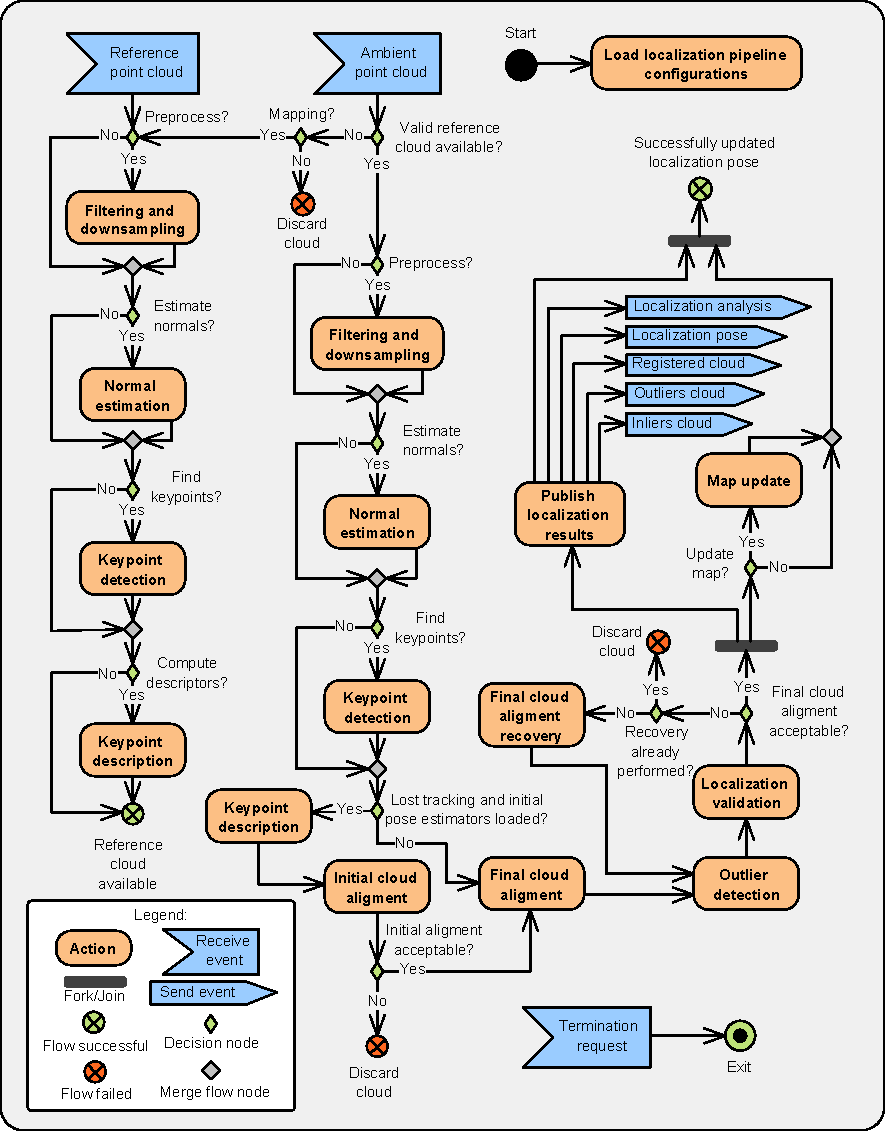
\includegraphics[width=0.5\textwidth]{localization-system/localization-system-overview}
	\caption{Localization system overview}
	\label{fig:localization-system_localization-system-overview}
\end{figure}
